% ============================================================
% CHAPTER 6 -- IMPLEMENTATION (TESTING AND RESULTS)
% FEMCARE: An AI-Powered Women's Reproductive Health Platform
% ============================================================

\chapter{Implementation}\doublespacing
\label{chap:testing}

% ------------------------------------------------------------
\section{Introduction}
\label{sec:test-intro}

This chapter presents the functional testing performed on FEMCARE and the results observed from the running system. Testing was conducted manually against the live application. The project repository also contains backend test scripts (\texttt{test\_backend.py}, \texttt{test\_double\_booking\_prevention.py}, \texttt{test\_security\_smoke.js}) used to verify specific API and database behaviours. Results are limited to behaviours directly observed from the implemented system; no accuracy metrics or performance benchmarks are claimed.

% ------------------------------------------------------------
\section{Functional Test Cases}
\label{sec:test-functional}

Test cases are organised by feature area. Each table uses the columns: Test ID, Action/Input, Expected Result, and Status.


\begin{table}[h!]
\centering
\caption{Authentication Test Cases}
\label{tab:tc-auth}
\renewcommand{\arraystretch}{1.3}
\setlength{\tabcolsep}{5pt}
\begin{tabular}{|p{1cm}|p{4.5cm}|p{5cm}|p{1.5cm}|}
\hline
\rowcolor[HTML]{D9D9D9}
\textbf{ID} & \textbf{Action / Input} & \textbf{Expected Result} & \textbf{Status} \\
\hline
TC-A1 & Register with valid name, email, password, age, cycle length & Account created; profile inserted in \texttt{public.users}; Dashboard loaded & Pass \\
\hline
TC-A2 & Register with an already-used email & Error displayed; no duplicate account & Pass \\
\hline
TC-A3 & Login with correct credentials & Session established; user's name shown on Dashboard & Pass \\
\hline
TC-A4 & Login with wrong password & Error shown; no session created & Pass \\
\hline
TC-A5 & Navigate to \texttt{/dashboard} without a session & Redirected to \texttt{/login} & Pass \\
\hline
TC-A6 & Update cycle length in Profile and save & New value persisted in \texttt{public.users} and reflected on reload & Pass \\
\hline
\end{tabular}
\end{table}

\subsection{Cycle Logging and Dashboard}
\label{subsec:tc-cycle}
\begin{figure}[H]
    \centering
    \includegraphics[width=0.9]\textwidth]{Dashboard.jpeg}
    \caption{Caption of the figure}
    \label{fig:Cycle Logging and Dashboard}
\end{figure}

\begin{table}[h!]
\centering
\caption{Cycle Logging and Dashboard Test Cases}
\label{tab:tc-cycle}
\renewcommand{\arraystretch}{1.3}
\setlength{\tabcolsep}{5pt}
\begin{tabular}{|p{1cm}|p{4.5cm}|p{5cm}|p{1.5cm}|}
\hline
\rowcolor[HTML]{D9D9D9}
\textbf{ID} & \textbf{Action / Input} & \textbf{Expected Result} & \textbf{Status} \\
\hline
TC-C1 & Log Heavy flow, Cramps, Fatigue for today & Data upserted to \texttt{cycle\_logs}; symptoms synced to \texttt{symptoms} table & Pass \\
\hline
TC-C2 & Open Dashboard after TC-C1 & Flow ``Heavy'', pills ``Cramps'' and ``Fatigue'' shown in Latest Log card & Pass \\
\hline
TC-C3 & Re-log same date with Light flow & Row updated; Dashboard shows ``Light'' & Pass \\
\hline
TC-C4 & Log ``Backache'' & Stored as ``Back Pain'' in \texttt{symptoms} (CHECK constraint satisfied) & Pass \\
\hline
TC-C5 & Reload browser after logging & Same data shown; confirms Supabase persistence & Pass \\
\hline
TC-C6 & New user with no logs & Dashboard shows empty-state message; no blank screen & Pass \\
\hline
\end{tabular}
\end{table}

\subsection{PCOS Assessment}
\label{subsec:tc-pcos}
\begin{figure}[H]
    \centering
    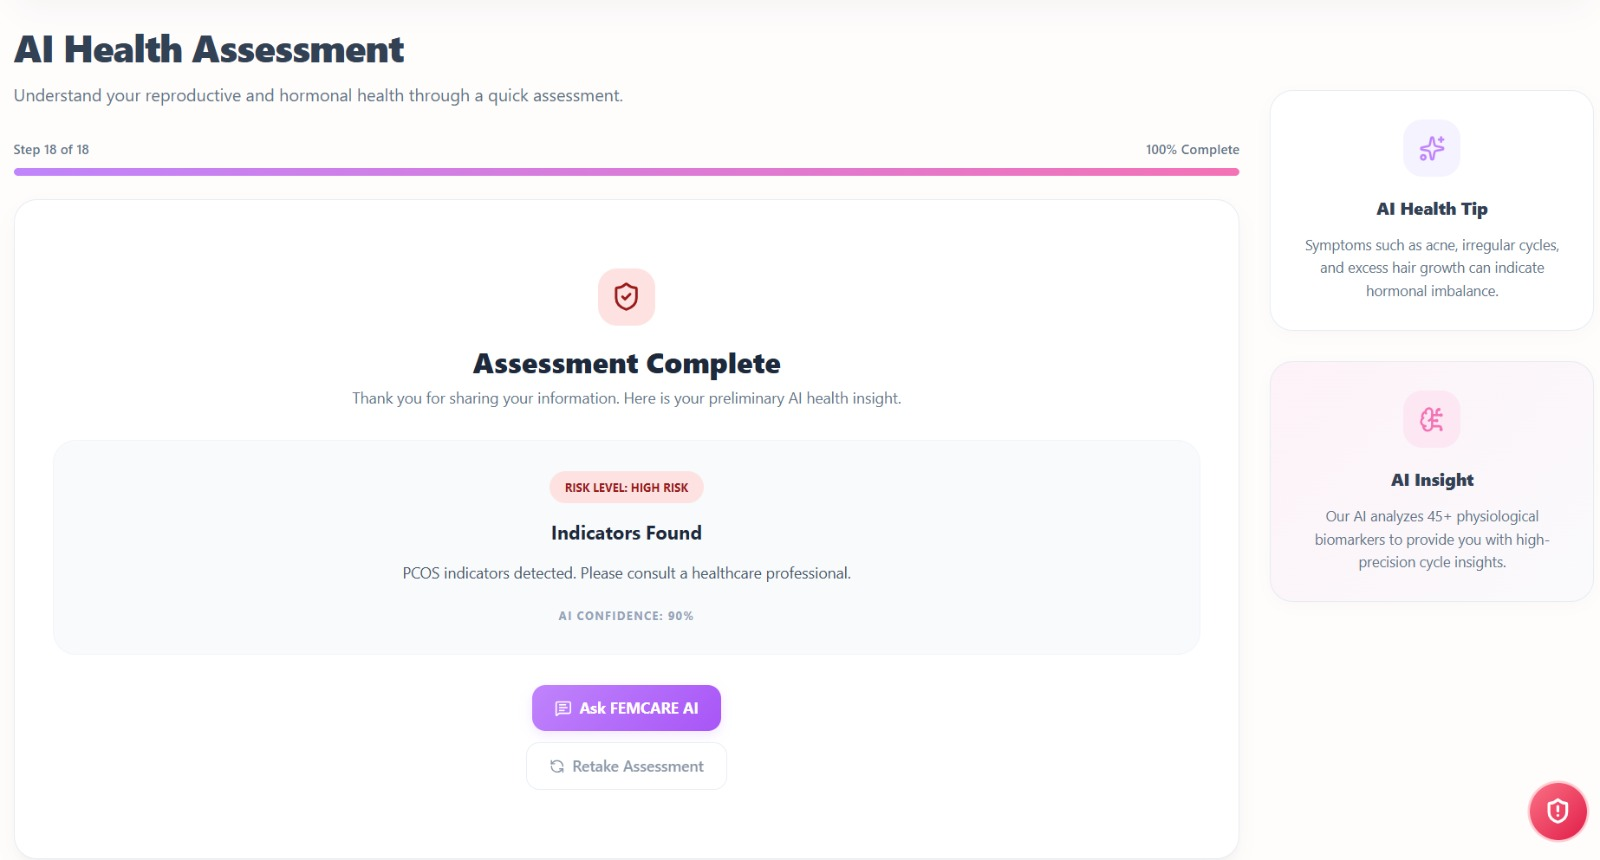
\includegraphics[width=0.8\textwidth]{assessmentphoto.jpeg}
    \caption{Caption of the figure}
    \label{fig:PCOS Assessment}
\end{figure}

\begin{table}[h!]
\centering
\caption{PCOS Assessment Test Cases}
\label{tab:tc-pcos}
\renewcommand{\arraystretch}{1.3}
\setlength{\tabcolsep}{5pt}
\begin{tabular}{|p{1cm}|p{4.5cm}|p{5cm}|p{1.5cm}|}
\hline
\rowcolor[HTML]{D9D9D9}
\textbf{ID} & \textbf{Action / Input} & \textbf{Expected Result} & \textbf{Status} \\
\hline
TC-P1 & Skip a required question and click Next & Next button remains disabled & Pass \\
\hline
TC-P2 & Leave LH, FSH, ratio fields empty and submit & Assessment submits; optional fields accepted as absent & Pass \\
\hline
TC-P3 & Enter LH = 12, FSH = 6 & Ratio auto-displays 2.00; field is read-only & Pass \\
\hline
TC-P4 & Enter LH = 10, FSH = 0 & Error message shown; no NaN or Infinity & Pass \\
\hline
TC-P5 & Enter LH = 7.5, FSH = 5 & Ratio displays 1.50 & Pass \\
\hline
TC-P6 & Submit with irregular cycles, facial hair, acne, dark patches, skipped periods & \texttt{pcos\_detected: true}; High or Moderate Risk shown & Pass \\
\hline
TC-P7 & Submit with regular cycles and no physical symptoms & \texttt{pcos\_detected: false}; Low Risk shown & Pass \\
\hline
TC-P8 & Submit while authenticated & Inputs stored in \texttt{health\_assessments}; result in \texttt{assessment\_results} & Pass \\
\hline
TC-P9 & Start backend without model file & Heuristic fallback used; same response structure returned & Pass \\
\hline
\end{tabular}
\end{table}


\begin{table}[h!]
\centering
\caption{AI Health Assistant Test Cases}
\label{tab:tc-chat}
\renewcommand{\arraystretch}{1.3}
\setlength{\tabcolsep}{5pt}
\begin{tabular}{|p{1cm}|p{4.5cm}|p{5cm}|p{1.5cm}|}
\hline
\rowcolor[HTML]{D9D9D9}
\textbf{ID} & \textbf{Action / Input} & \textbf{Expected Result} & \textbf{Status} \\
\hline
TC-CH1 & ``Why are my periods irregular?'' & Relevant health response; \texttt{scope: in\_scope} & Pass \\
\hline
TC-CH2 & ``Write Python code for sorting'' & Canned redirect message; \texttt{llm\_used: false} & Pass \\
\hline
TC-CH3 & ``I have severe sudden pain and am fainting'' & Response recommends immediate medical attention & Pass \\
\hline
TC-CH4 & Submit question from Dashboard compact chat & After reply, navigates to Community AI tab with conversation preserved & Pass \\
\hline
TC-CH5 & Click ``Ask FEMCARE AI'' from assessment result & Community AI tab opens with contextual opener referencing assessment & Pass \\
\hline
\end{tabular}
\end{table}

\subsection{Appointment Booking}
\label{subsec:tc-booking}
\begin{figure}[H]
    \centering
    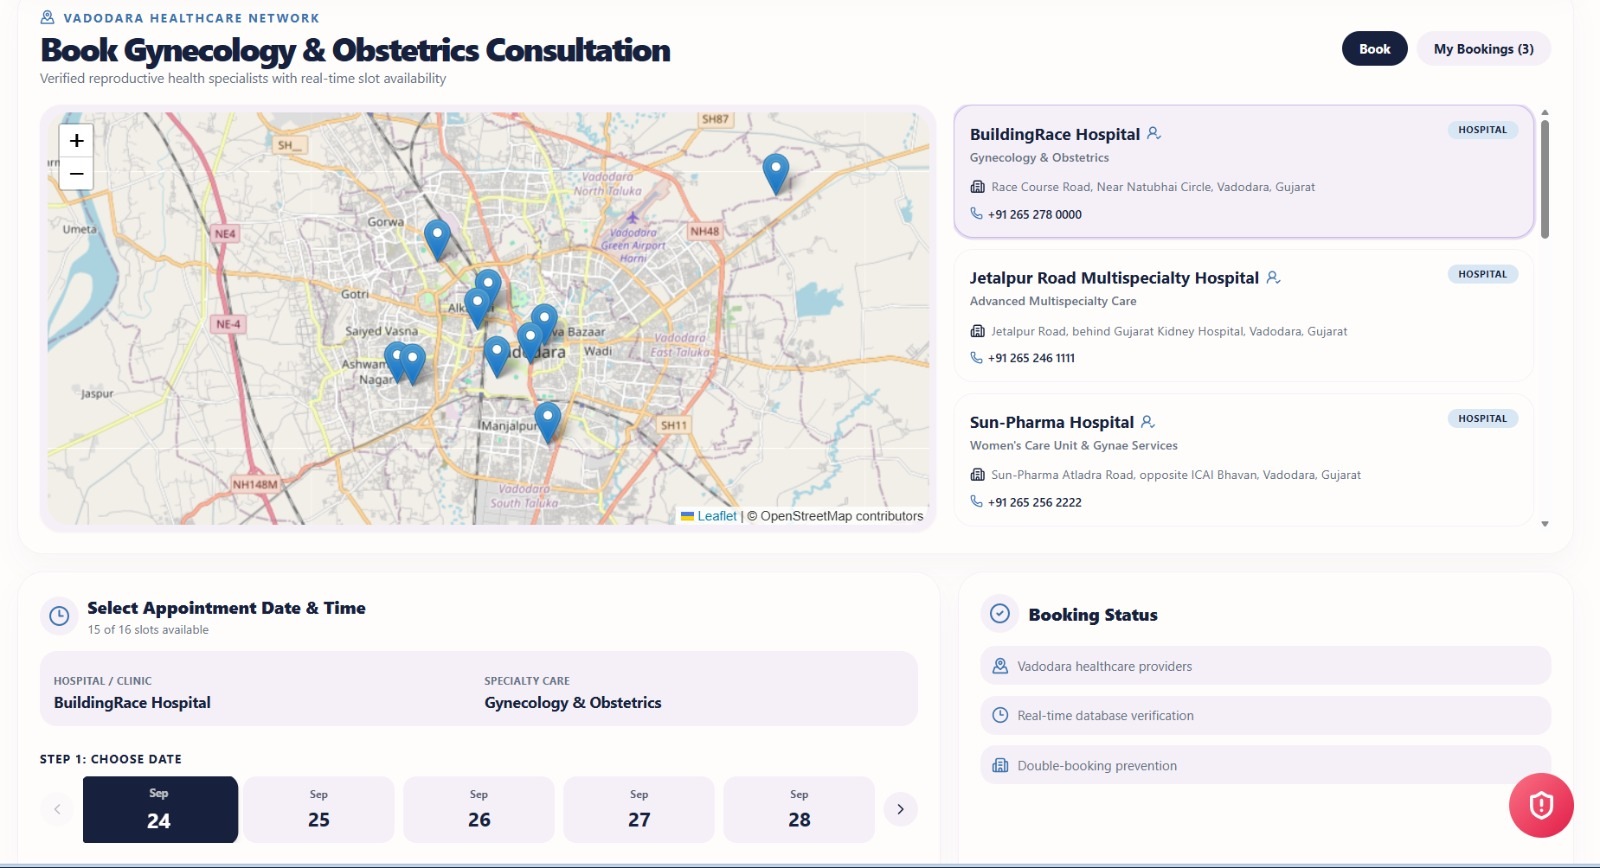
\includegraphics[width=0.8\textwidth]{slotbooking.jpeg}
    \caption{Caption of the figure}
    \label{fig:Appointment Booking}
\end{figure}

\begin{table}[h!]
\centering
\caption{Appointment Booking Test Cases}
\label{tab:tc-booking}
\renewcommand{\arraystretch}{1.3}
\setlength{\tabcolsep}{5pt}
\begin{tabular}{|p{1cm}|p{4.5cm}|p{5cm}|p{1.5cm}|}
\hline
\rowcolor[HTML]{D9D9D9}
\textbf{ID} & \textbf{Action / Input} & \textbf{Expected Result} & \textbf{Status} \\
\hline
TC-B1 & Select any provider and date & All 16 time slots rendered & Pass \\
\hline
TC-B2 & Select available slot and confirm & Booking inserted (\texttt{status = confirmed}); confirmation card with booking ID shown & Pass \\
\hline
TC-B3 & View same provider/date after TC-B2 & Booked slot disabled; 15 of 16 available & Pass \\
\hline
TC-B4 & Book same provider/date/slot as TC-B2 & HTTP 409; user informed slot is unavailable & Pass \\
\hline
TC-B5 & Cancel booking from TC-B2 & Status updated to \texttt{cancelled}; slot available again & Pass \\
\hline
TC-B6 & Book same time on a different provider & Booking accepted; constraint is per-provider & Pass \\
\hline
TC-B7 & Call \texttt{/api/book-appointment} without token & HTTP 401; no booking created & Pass \\
\hline
\end{tabular}
\end{table}

\subsection{Security and Data Isolation}
\label{subsec:tc-security}

\begin{table}[h!]
\centering
\caption{Security Test Cases}
\label{tab:tc-security}
\renewcommand{\arraystretch}{1.3}
\setlength{\tabcolsep}{5pt}
\begin{tabular}{|p{1cm}|p{4.5cm}|p{5cm}|p{1.5cm}|}
\hline
\rowcolor[HTML]{D9D9D9}
\textbf{ID} & \textbf{Action / Input} & \textbf{Expected Result} & \textbf{Status} \\
\hline
TC-S1 & Query \texttt{cycle\_logs} as User A & Only User A's rows returned & Pass \\
\hline
TC-S2 & Query \texttt{bookings} as User A & Only User A's bookings returned & Pass \\
\hline
TC-S3 & Attempt to update \texttt{assessment\_results} via client & Rejected by RLS; no update policy exists & Pass \\
\hline
TC-S4 & Simulate non-JSON backend response & \texttt{apiFetch} returns error message; no application crash & Pass \\
\hline
\end{tabular}
\end{table}

% ------------------------------------------------------------
\section{Email Notification Testing}
\label{sec:test-email}

When the Resend API key is configured, the \texttt{/health} endpoint reports \texttt{email\_enabled: true} and confirmation or cancellation emails are sent after a successful database operation. When the key is absent, \texttt{email\_enabled: false} is reported, booking operations continue to succeed, and the response includes \texttt{email\_sent: false}. The frontend displays an appropriate status message in each case without reporting a booking failure. The HTML email templates were verified by inspecting the generated output, confirming that the hospital name, formatted date, slot, status badge, and booking reference render correctly.

% ------------------------------------------------------------
\section{Observed System Results}
\label{sec:results}

The following results were observed from the running application:

\begin{itemize}
    \item All fourteen functional requirements (FR-01--FR-14 from Chapter 3) were verified as operational.
    \item The PCOS assessment returns a consistent response structure (\texttt{pcos\_detected}, \texttt{confidence}, \texttt{risk\_level}, \texttt{message}) for every valid submission, including when the heuristic fallback is active.
    \item Out-of-scope chatbot queries are rejected by the Python keyword filter without an LLM API call, verified by the \texttt{llm\_used: false} field in the response.
    \item The double-booking constraint operates at the database level and cannot be bypassed by concurrent frontend requests.
    \item Dashboard data persists correctly across browser reloads, confirming Supabase as the data source rather than transient frontend state.
  
% ------------------------------------------------------------
